\RequirePackage{fix-cm}
\documentclass[smallextended]{svjour3}
\smartqed

\usepackage{graphicx}
\usepackage{url}
\usepackage{xcolor}
\usepackage{booktabs}
\usepackage{multirow}
\usepackage{amsmath,amssymb,amsfonts}
\graphicspath{{figures/}}
\emergencystretch=2em
\def\UrlBreaks{\do\/\do-\do_}
\Urlmuskip=0mu plus 1mu\relax

\journalname{Medical \& Biological Engineering \& Computing}


\begin{document}

\title{From Endoscopic Image Sequences to a Simulable Soft-Tissue Digital Twin: Gaussian Surface Tracking and Force-Scale-Aware Mechanical Inversion}
\titlerunning{Simulable soft-tissue digital twin}

\author{Ranyang Li \and Haotian Ma \and Zhipeng Lin \and Nan Wei}
\authorrunning{R. Li et al.}

\institute{R. Li \and H. Ma \at
Henan University of Technology, Zhengzhou 450001, China\\
\email{lry@haut.edu.cn}
\and
Z. Lin \at
Beihang University, Beijing 100191, China
\and
N. Wei \at
Henan Provincial People's Hospital, Zhengzhou 450003, China}

\date{}
\maketitle

\begin{abstract}
Endoscopic reconstruction estimates
appearance and surface motion but does not by itself provide a mechanically
valid, simulable tissue model. We propose a soft-tissue digital-twin
framework that converts endoscopic images into a co-registered Gaussian
surface, optical material representation, displacement field, and
force-aware volumetric mechanics. A canonical anisotropic Gaussian field
is reconstructed with depth-valid, instrument-excluded supervision and
tracked by fixed primitive identities using graph regularization,
constant-velocity initialization, and divergence rollback. An explicit
Gaussian-to-tetrahedral interface transfers surface observations to a
differentiable Neo-Hookean solver. Known forces permit modulus inversion;
without force sensing, a derived force-scale relation limits inference to
stiffness contrast. Each parameter is labelled measured, estimated, or
assumed and accompanied by uncertainty. Evaluation combines two EndoNeRF
sequences, two SCARED keyframes, 60 finite-element scenarios, six phantom
acquisitions, and one clinical computed-tomography case. On a strict
28-frame holdout, tissue peak signal-to-noise ratio/structural similarity were 16.7 dB/0.564 for the present method and 36.6 dB/0.939 for EndoGaussian. Across 60 finite-element scenarios, median errors were 9.6\% for background modulus, 32.0\% for inclusion modulus, and 32.4\% for contrast. Phantom contrast was $3.80\times$ versus
$3.56\times$ by compression testing. The contribution is a traceable
observation-to-simulation interface; absolute tissue modulus still
requires measured force.
\keywords{digital twin \and soft tissue \and endoscopic reconstruction
\and elasticity inversion \and parameter provenance \and biomechanics}
\end{abstract}


\section{Introduction}
\label{sec:intro}

Surgical rehearsal and patient-specific intervention planning require more
than a visual reconstruction: the virtual tissue must also respond to a
prescribed load through a mechanically interpretable forward model
\cite{landig2025,laubenbacher2024}. Endoscopic reconstruction can recover
appearance, surface geometry, and motion, but these observations do not by
themselves identify Young's modulus, Poisson's ratio, or stress. This work
therefore addresses the interface between endoscopic observation and a
simulable soft-tissue representation.

The central difficulty is evidential. Geometry and reflectance are
constrained by images and auxiliary depth, whereas elasticity is constrained
only through deformation under a known or otherwise calibrated load. Values
copied from a tissue table remain assumptions rather than patient-specific
measurements. The proposed twin consequently attaches a provenance state
(measured, estimated, or assumed) and uncertainty to each physical
parameter, so that simulated stress and strain can be interpreted according
to the evidence that supports them.


\begin{figure}[htbp]
\centering
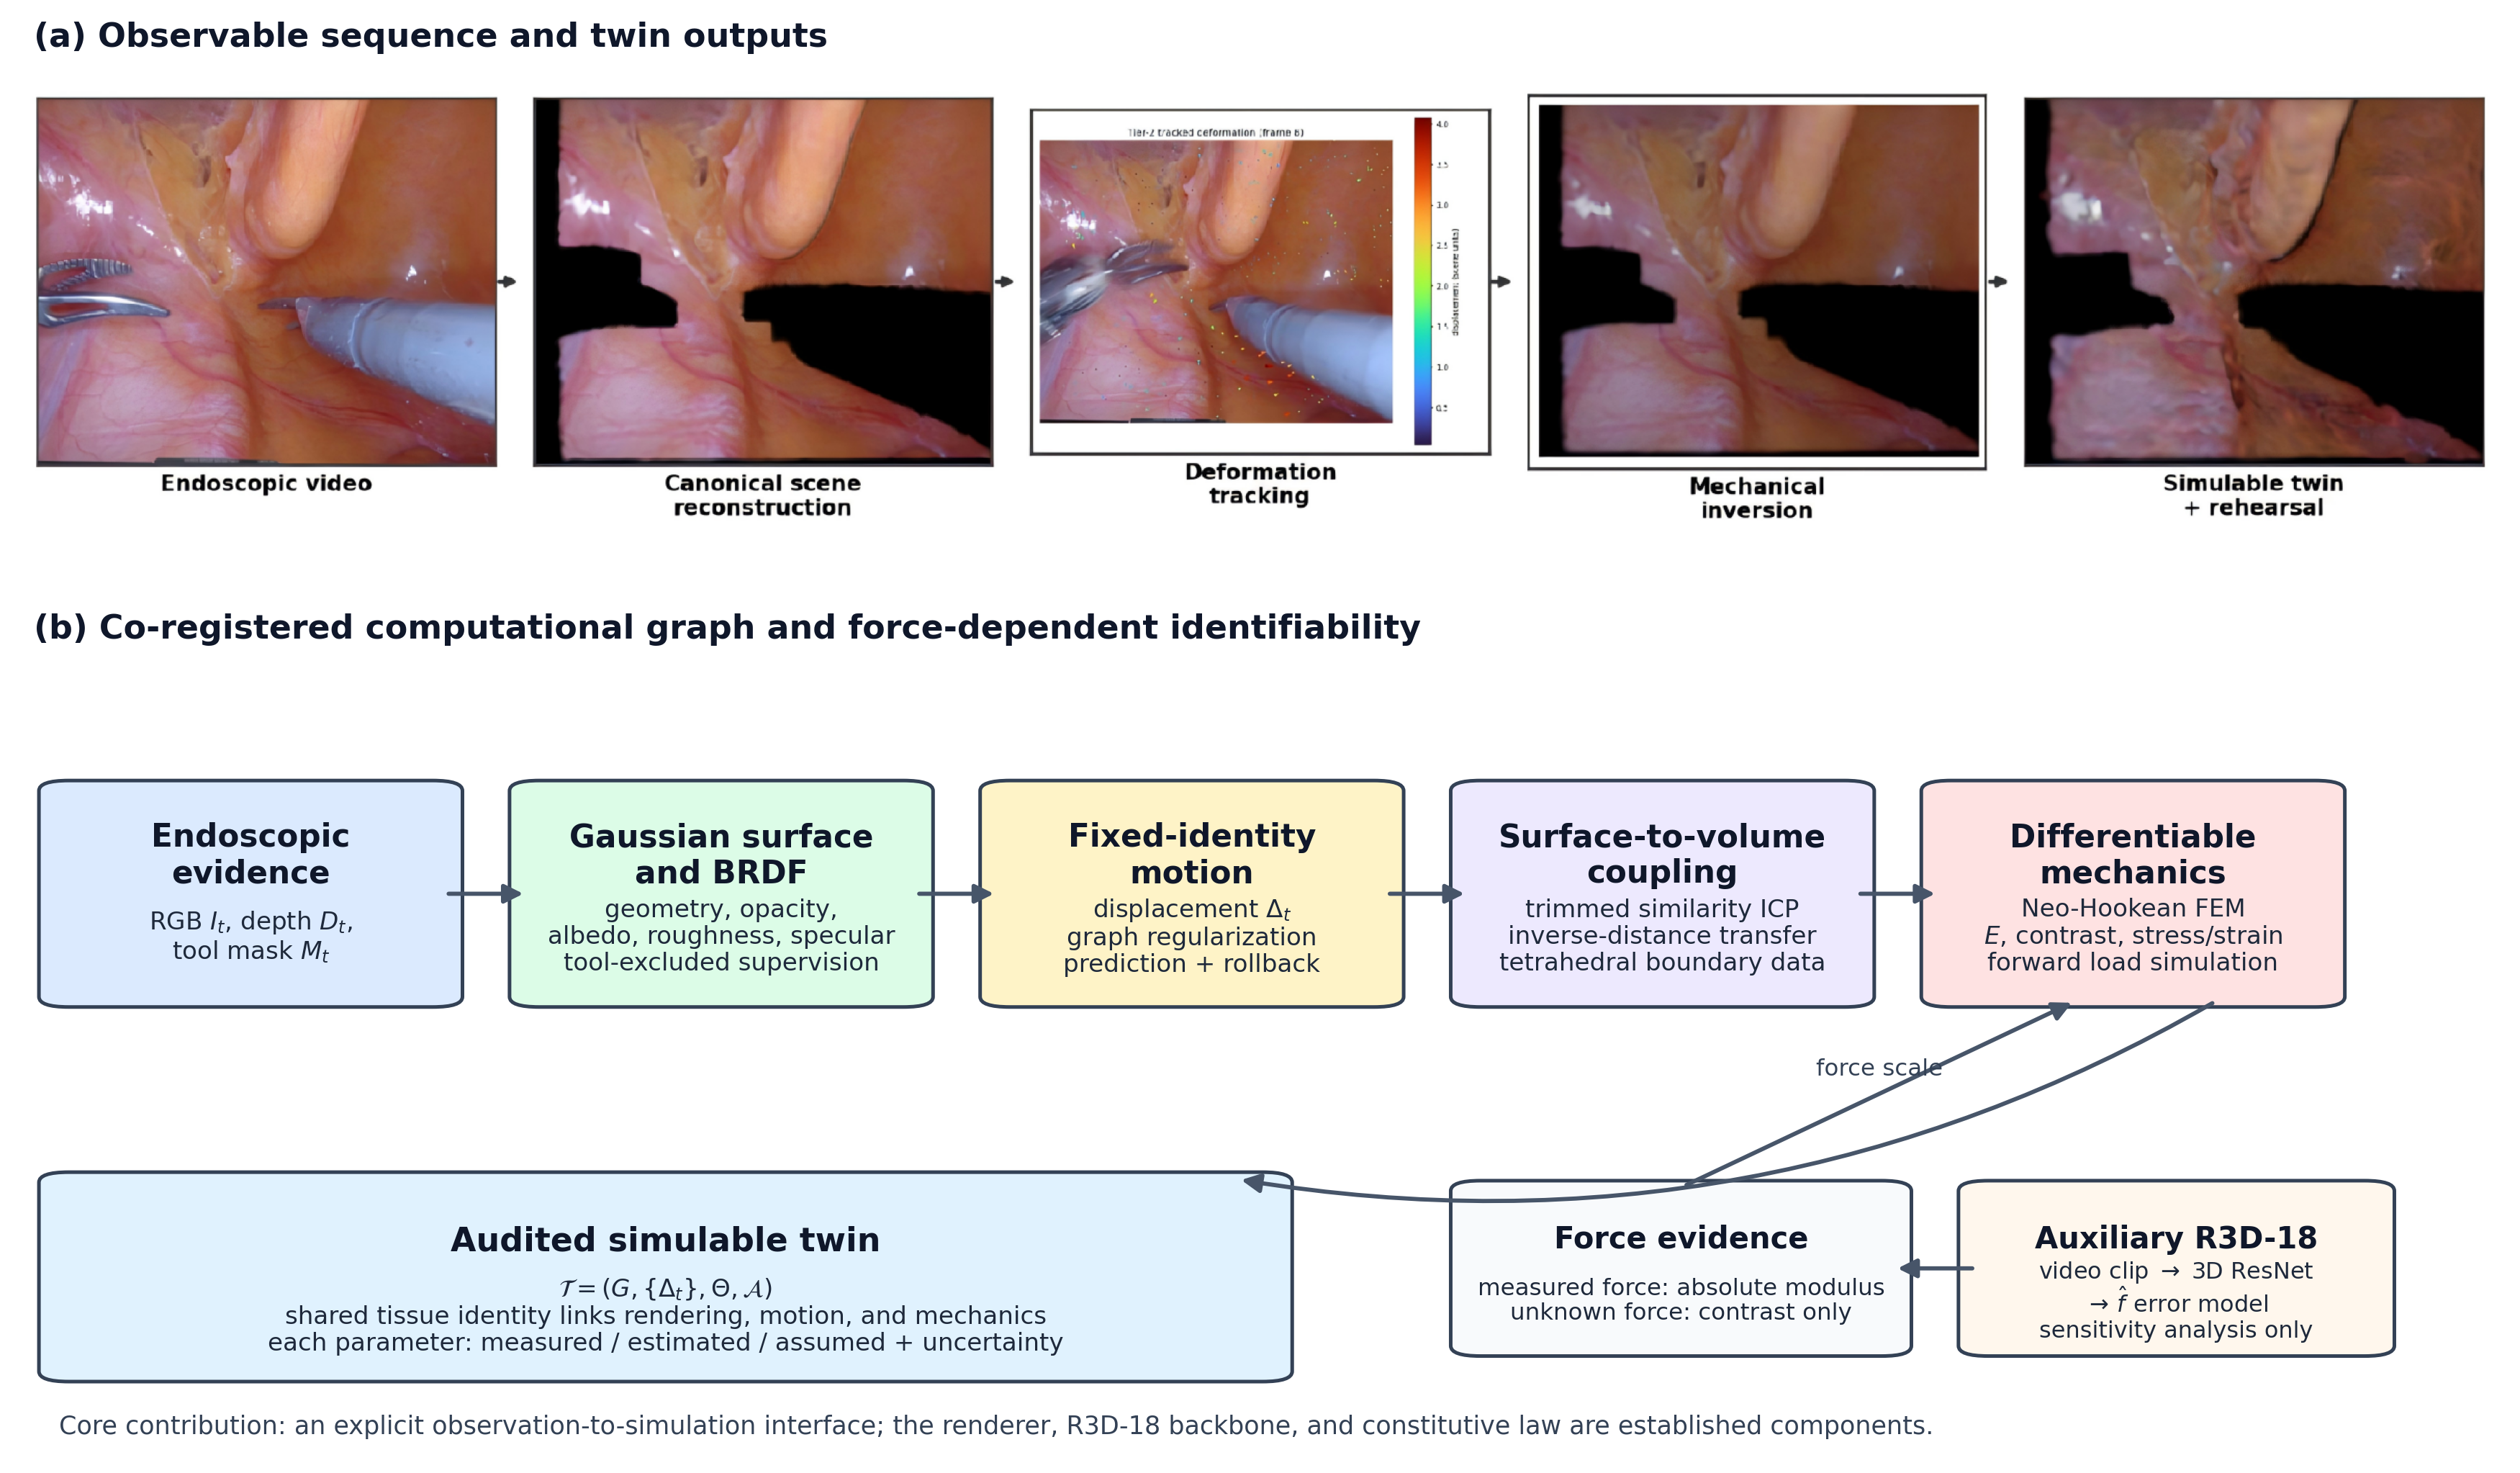
\includegraphics[width=\textwidth]{fig_overall_framework.png}
\caption{Overall soft-tissue digital-twin framework. (a) Endoscopic
observations are reconstructed, tracked, mechanically parameterized, and
driven forward for rehearsal. (b) The computational graph keeps Gaussian
surface identity fixed while transferring displacement to a separate
tetrahedral discretization. Force evidence determines whether absolute
modulus or only stiffness contrast is identifiable. The compact R3D-18
branch summarizes the auxiliary estimator used only to define a
force-error model; it is external to the core twin.}
\label{fig:overall_framework}
\end{figure}


\subsection{Related work and methodological gap}
EndoNeRF \cite{endonerf} and EndoSurf \cite{endosurf} reconstruct
deforming endoscopic scenes with neural radiance or signed-distance fields.
EndoGaussian \cite{endogaussian} uses anisotropic Gaussians and a learned
spatiotemporal deformation field to achieve high-quality, real-time
novel-view synthesis. Related inverse-rendering methods decompose geometry,
lighting, and bidirectional reflectance \cite{gsir2024,relightable3dgs},
while deformable SLAM and robust pose estimation address camera motion
\cite{defslam,hayoz2023}. These methods establish visual reconstruction
but do not produce force-conditioned tissue mechanics.

Physics-aware neural representations address complementary parts of the
problem. PAC-NeRF identifies material parameters from multi-view motion
under known loading \cite{pacnerf}; PhysDreamer estimates relative
stiffness without an absolute force scale \cite{physdreamer}; and
PhysGaussian and Spring-Gaus couple visual primitives to prescribed or
learned dynamics \cite{physgaussian,springgaus}. Quasi-static
elastography likewise shows that deformation can support stiffness contrast
under a shared-load approximation, while absolute modulus requires force
information \cite{ophir1991,wells2011,sigrist2017}. No compared method
provides the complete endoscopic observation-to-volumetric-simulation
interface together with explicit parameter provenance.

We propose a co-registered representation
$\mathcal{T}=(G,\{\Delta_t\},\Theta,\mathcal{A})$. A canonical
Gaussian field $G$ stores geometry and Cook--Torrance optical material;
fixed primitive identities carry displacement $\Delta_t$ through time; an
explicit alignment and interpolation map transfers surface observations to
a tetrahedral Neo-Hookean model with parameters $\Theta$; and
$\mathcal{A}$ records provenance and uncertainty. Constant-velocity
initialization, graph regularization, and divergence rollback stabilize
tracking. A force-scale analysis establishes that a common scaling of force
and regional moduli leaves equilibrium displacement and stiffness contrast
unchanged, which prevents unsupported absolute-modulus claims when force is
not measured.

The evaluation uses two EndoNeRF sequences, two SCARED keyframes, all 60
scenarios of a four-load finite-element benchmark, six ultrasound-phantom
acquisitions with compression-test references, and one de-identified
clinical CT geometry. Under the same 28-frame holdout, EndoGaussian reaches
36.6 dB tissue PSNR and 0.939 tissue SSIM, compared with 16.7 dB and 0.564
for the present representation; reconstruction superiority is therefore
not claimed. The complete FEM campaign gives median errors of 9.6\% for
background modulus, 32.0\% for inclusion modulus, and 32.4\% for contrast.
The phantom contrast is 3.80$\times$ versus 3.56$\times$ by compression
testing. These experiments test the integrated twin and its identifiability
limits rather than clinical effectiveness.

\section{Methods}
\label{sec:method}

\subsection{Study design, data, and evaluation}
This computational methods study separates visual reconstruction,
surface tracking, known-force inversion, force-uncertain contrast
estimation, and geometry-to-volume coupling. EndoNeRF contributes two RGB
sequences (63 and 156 frames) with auxiliary depth and instrument masks;
SCARED contributes two stereo keyframes with metric depth
\cite{endonerf,scared}. The synthetic benchmark contains 60
Neo-Hookean scenarios and four loads with ground-truth regional moduli,
measured forces, and noisy surface motion. The physical dataset contains
six ultrasound indentation acquisitions and independent compression-test
moduli \cite{etsphantom}. A single de-identified hospital CT case is used
only to construct a patient-specific tetrahedral geometry.

The strict reconstruction split excludes frames satisfying
$(t-1)\bmod 8=0$ from both methods. PSNR and SSIM use identical source
images and masks; tissue SSIM averages the local 11-by-11 SSIM map only
over tissue pixels. Mechanical accuracy is reported as relative modulus
error, contrast error, and held-out-load displacement error. FEM scenarios
are processed in lexical order with a frozen 20-iteration inversion.
Medians, means, interquartile ranges, and per-case values are reported; the
phantom median uses a nonparametric bootstrap 95\% confidence interval.

\subsection{Digital-twin representation}
The twin is
$\mathcal{T}=(G,\{\Delta_t\},\Theta,\mathcal{A})$, where $G$ is the
canonical Gaussian geometry and optical material, $\Delta_t$ is
fixed-identity surface displacement, $\Theta$ contains the mechanical
parameters and forward operator, and $\mathcal{A}$ maps every parameter to
its provenance and uncertainty. Inputs are images $I_t$, depth $D_t$, and
tool masks $M_t$. A twin is considered simulable when the mechanical
operator maps a new load to volumetric displacement and derived stress or
strain; it is considered audited only when every parameter has a
provenance tag.

\subsection{Canonical scene reconstruction}
\label{sec:tier1}
Reconstruction builds $G$. Each Gaussian $g_i$ stores a position
$\mathbf{x}_i \in \mathbb{R}^3$, an anisotropic covariance
$\Sigma_i = Q(q_i)\,\mathrm{diag}(s_i^2)\,Q(q_i)^{\top}$ with rotation
quaternion $q_i$ and scale $s_i$, an opacity $o_i \in [0,1]$, a unit normal
$\mathbf{n}_i$, and BRDF parameters $(\rho_d, \rho_s, \alpha, m, a)$. A
softmax budget regularizes the relative lobe weights by a partition of
unity,
\begin{equation}
\rho_d + \rho_s + a = 1, \qquad \rho_d,\rho_s,a \ge 0,
\label{eq:budget}
\end{equation}
which prevents unconstrained growth of these fitted coefficients; it is
not by itself a proof of global energy conservation under the discretized
lighting model. Images are formed by front-to-back alpha compositing,
\begin{equation}
\hat{I} = \sum_{i=1}^{N} c_i\,\alpha_i \prod_{j<i}(1-\alpha_j),
\label{eq:render}
\end{equation}
where $c_i$ is the shaded color of $g_i$ and $\alpha_i$ its projected
opacity. The shaded color follows a Cook--Torrance microfacet BRDF
\cite{cooktorrance} split into a diffuse and a specular lobe,
\begin{equation}
c_i = \underbrace{\frac{\rho_d}{\pi}\,E_d}_{\text{diffuse}}
+ \underbrace{\rho_s\,\frac{D(\alpha)\,G_s\,F}{4\,(\mathbf{n}\cdot\mathbf{l})(\mathbf{n}\cdot\mathbf{v})}}_{\text{specular}},
\label{eq:cooktorrance}
\end{equation}
where $E_d$ is the diffuse irradiance, $D(\alpha)$ the GGX normal
distribution, $G_s$ the Smith geometry term, $F$ the Schlick Fresnel term,
$\mathbf{l}$ the light direction, and $\mathbf{v}$ the view direction. The
dot products in the denominator are clamped away from zero on visible
front-facing samples, and the specular term is zero for back-facing
samples. The
highlight-free diffuse image is obtained by setting the specular lobe to
zero.

A key endoscopic adaptation concerns the supervision mask. The EndoNeRF
\texttt{masks/} channel marks \emph{tools}, not tissue, and tools have no
valid depth. We therefore define the tissue pixel set as
\begin{equation}
\Omega = \{(u,v) : D(u,v) > \epsilon \} \setminus M,
\label{eq:mask}
\end{equation}
with $\epsilon$ a small depth-validity threshold, and supervise only on
$\Omega$. Supervising on the tool mask instead of $\Omega$ degrades
reconstruction by ${\sim}25$\,dB (Table~\ref{tab:ablation}). The reconstruction
objective is
\begin{equation}
\mathcal{L}_1 = \lambda_{ph}\,\mathcal{L}_{photo} + \lambda_d\,\mathcal{L}_{depth} + \lambda_\alpha\,\mathcal{L}_{\alpha},
\label{eq:tier1loss}
\end{equation}
with non-negative weights $\lambda_{ph},\lambda_d,\lambda_\alpha$, a masked
$L_1 + 0.5\,L_2$ photometric term $\mathcal{L}_{photo}$ on $\Omega$, a
depth $L_1$ term $\mathcal{L}_{depth}$ on $\Omega$, and an alpha
binary-cross-entropy term
$\mathcal{L}_{\alpha}$ toward the tissue mask. Lighting is an
endoscope-co-located directional light plus a strong ambient
spherical-harmonic lobe, so appearance approximates albedo; a learnable
exposure closes the residual gap.

\subsection{Deformation tracking}
\label{sec:tier2}
Tracking estimates $\{\Delta_t\}$ as a per-Gaussian displacement
$\Delta_t \in \mathbb{R}^{N \times 3}$ on the canonical topology, keeping
correspondences fixed across time. Fixed correspondence is what
distinguishes a twin from a per-frame rebuild: the same primitive is
followed through time, so its trajectory is a boundary condition. Naive
inertia-only tracking (penalizing $\|\Delta_t - \Delta_{t-1}\|^2$)
occasionally diverges on ambiguous frames. We therefore optimize
\begin{align}
\Delta_t^* = \arg\min_{\Delta}\ \ & \mathcal{L}_{photo}(\Delta)
+ \lambda_s \sum_{i=1}^{N} \big\| \Delta_i - \bar{\Delta}_{\mathcal{N}(i)} \big\|^2 \nonumber\\
& + \lambda_a \big\| \Delta - 2\Delta_{t-1} + \Delta_{t-2} \big\|^2,
\label{eq:track}
\end{align}
initialized from the constant-velocity extrapolation
$\Delta_t^{(0)} = 2\Delta_{t-1} - \Delta_{t-2}$. The second term is a
$k$-nearest-neighbor Laplacian smoothness over the Gaussian graph; the
quantity $\bar{\Delta}_{\mathcal{N}(i)}$ is the mean displacement of the
neighbors of primitive $i$. The third term is an acceleration prior that
penalizes changes in velocity rather
than velocity itself. A per-frame step cap constrains
$N^{-1}\sum_i\|\Delta_{t,i}\|_2$ to at most three times the running median
of preceding displacement magnitudes, and
a divergence rollback repeats optimization at half the learning rate when
the final loss exceeds three times the preceding-frame loss. If the
criterion remains unmet, $\Delta_{t-1}$ is retained and the frame is
flagged. The output is a sequence of replayable boundary conditions.

\subsection{Coupling tracked Gaussians to mechanics}
\label{sec:coupling}
The optical and mechanical computations use different discretizations.
Gaussian primitives represent the observed surface, whereas the FEM
benchmark uses a tetrahedral volume mesh. Coupling is therefore performed
through surface displacement rather than by treating Gaussians as finite
elements.

For an uninstrumented endoscopic sequence, canonical Gaussian positions
are partitioned into four spatial regions $C_r$ by $k$-means. For region $r$,
the mean displacement magnitude is
\begin{equation}
d_r = \frac{1}{|C_r|}\sum_{i\in C_r}\|\Delta_{t,i}\|_2 .
\label{eq:relative_displacement}
\end{equation}
Under the common-load approximation used in quasi-static elastography, a
relative-stiffness proxy is
\begin{equation}
\kappa_r = \frac{\max_s d_s}{d_r+\epsilon_d},
\label{eq:relative_stiffness}
\end{equation}
where $\epsilon_d=10^{-9}$ in the displacement units prevents division by
zero and the most compliant region has $\kappa=1$. This calculation
provides regional contrast only. The
absolute modulus remains the tissue prior because the endoscopic sequence
does not contain a force measurement.

For known-force benchmark experiments, the observed displacement is
defined on surface nodes $\Gamma_{obs}$ of the tetrahedral mesh. The FEM
parameters are optimized so that simulated surface displacement matches
these observations. The two settings evaluate complementary outputs:
co-registered contrast on tracked Gaussians and absolute-modulus inversion
on a force-calibrated volumetric mesh.

For the patient-specific geometry experiment, a binary CT liver mask is
block-reduced and each occupied voxel is divided into six tetrahedra with
shared nodes. The Gaussian surface is initialized to the volume boundary
by principal-axis alignment and refined by trimmed similarity iterative
closest point registration. For every covered volume-boundary node, the
four nearest transformed Gaussians define inverse-distance weights
$w_{ij}$, and tracked displacement is transferred as
\begin{equation}
\begin{aligned}
u_j^{obs} &= \sum_{i\in\mathcal{N}_4(j)} w_{ij}\Delta_i,\\
w_{ij} &=
\frac{(d_{ij}+\varepsilon)^{-1}}
{\sum_{k\in\mathcal{N}_4(j)}(d_{kj}+\varepsilon)^{-1}} .
\end{aligned}
\label{eq:surface_volume_map}
\end{equation}
Only boundary nodes whose nearest Gaussian lies within 5\% of the volume
diagonal are marked as observed. This map preserves separate optical and
mechanical discretizations while providing explicit correspondences for
boundary conditions. Because the Gaussian and CT surfaces are from
different subjects and the CT spacing metadata are unavailable, the
experiment validates the computational interface, not anatomical
registration.

\subsection{Mechanical parameter inversion with known force}
\label{sec:tier3}
For known-force cases, mechanical inversion defines $\Theta$ and the
forward operator $\mathcal{S}$. Soft tissue
is modeled as a quasi-static continuum in equilibrium,
\begin{equation}
R(u; E, \nu, f) = f_{int}(u; E, \nu) - f = 0,
\label{eq:equilibrium}
\end{equation}
where $f_{int}$ is the internal elastic force and $f$ is the applied load.
We invert $E$ by gradient descent through a differentiable forward
solver,
\begin{equation}
E^* = \arg\min_{E} \sum_{t} \big\| u(E, \nu, f_t) - u_t^{obs} \big\|_{\Gamma_{obs}}^{2} + \gamma\,\mathcal{R}(E),
\label{eq:inversion}
\end{equation}
where $u(E,\nu,f_t)$ is the simulated displacement under load $f_t$,
$u_t^{obs}$ the observed deformation, $\gamma \ge 0$ a regularization
weight, and $\mathcal{R}(E)$ a regularizer
(log-normal prior plus spatial smoothness). Two forward models are used: a
mass--spring lattice (structural and shear springs with stiffness
$k = E\,h$, $h$ the lattice spacing) for synthetic closed-loop studies, and
a differentiable Neo-Hookean FEM \cite{holzapfel2000,ogden1997,fung1993}
with strain-energy density
\begin{equation}
\Psi(F) = \frac{\mu}{2}\big(\mathrm{tr}(F^{\top}F) - 3\big) - \mu\,\log J + \frac{\lambda}{2}(\log J)^2,
\label{eq:neohookean}
\end{equation}
where $F$ is the deformation gradient, $J = \det F$, and
$\mu = E/(2(1+\nu))$, $\lambda = E\nu/((1+\nu)(1-2\nu))$ are the Lam\'e
parameters. The FEM solve uses Newton iteration with load stepping and warm
starts, and gradients are obtained by the implicit-function theorem through
the equilibrium. A kPa-scale log-normal tissue database (liver, fat,
muscle, skin, tumor; ) with near-incompressible $\nu$
and constitutive-model tags (Neo-Hookean / Mooney--Rivlin
\cite{rivlin1948} / Ogden \cite{ogden1997}) provides priors; the tissue
class is selected by heuristic optical features (colour and specular
response). This classification selects a prior category and does not
directly determine the mechanical values.



\subsection{Force-scale propagation}
\label{sec:forcescale}
The following result provides the theoretical basis for reporting
stiffness contrast as a force-scale-independent estimated quantity.

At fixed Poisson ratio, the Neo-Hookean internal force is linear in Young's modulus. Scaling all regional moduli and the applied force by the same factor therefore leaves equilibrium displacement unchanged, while regional stiffness contrast is invariant to that scale.


\subsection{Parameter provenance}
\label{sec:uq}
\begin{definition}[Parameter provenance]
\label{def:provenance}
A physical parameter $\theta$ carries a provenance tag
$\tau(\theta) \in \{\text{measured}, \text{estimated}, \text{assumed}\}$ and
a confidence $c(\theta) \in [0,1]$. A parameter is \emph{measured} when it
is acquired directly by a calibrated sensor, \emph{estimated} when it is
inferred by reconstruction or inverse simulation, and \emph{assumed} when
it is taken from a tissue-class table without case-specific evidence.
\end{definition}

Young's modulus uses a log-normal prior
$\log E \sim \mathcal{N}(\mu_0, \sigma_0^2)$, appropriate because tissue
stiffness spans orders of magnitude and must stay positive. A
Gaussian--Gaussian update combines the prior with deformation evidence in
closed form,
\begin{align}
\sigma_{post}^{-2} &= \sigma_0^{-2} + \sigma_{obs}^{-2}, \nonumber\\
\mu_{post} &= \sigma_{post}^{2}\left(
\frac{\mu_0}{\sigma_0^{2}} + \frac{\mu_{obs}}{\sigma_{obs}^{2}}
\right).
\label{eq:bayes}
\end{align}
where $(\mu_{obs}, \sigma_{obs})$ summarize the deformation evidence. The
confidence is the fractional posterior narrowing,
$c = 1 - \sigma_{post}/\sigma_0$. For uncertainty propagation, a Laplace
approximation $p(\log E \mid \text{data}) \approx \mathcal{N}(\log E^*, H^{-1})$
with $H$ the Hessian of the negative log-posterior at the optimum is
sampled by Monte Carlo through the simulator to a 95\% prediction interval.

\subsection{Twin synchronization and simulation}
\label{sec:sync}
A digital twin is not a one-shot reconstruction but a continuously updated
copy \cite{landig2025}. Synchronization is the tracking loop: as each new
frame arrives, the tracker updates $\{\Delta_t\}$ on the fixed canonical
topology, and mechanical inversion can reuse the accumulated deformation as
additional inversion evidence.
Once constructed, the twin is used by driving $\mathcal{S}$ with new loads:
given a planned instrument trajectory $\{f_t^{plan}\}$, the simulator
produces the predicted deformation $\{u(E^*, \nu, f_t^{plan})\}$, which can
be rendered through the canonical field for visual rehearsal or post-processed
for quantities of interest (contact force, strain energy density, margin
strain). The audit modulates how these predictions are presented:
predictions are accompanied by intervals propagated from the corresponding
parameter uncertainties.

\begin{remark}[Optimization and learned components]
\label{rem:networkfree}
The Gaussian field is optimized as a set of per-primitive parameters, the
renderer is differentiable, and mechanical inversion optimizes physical
parameters through the simulator. The auxiliary R3D-18 force estimator is
external to the twin and is used only to define the force-error model in
Sec.~\ref{sec:forcescale}.
\end{remark}

\section{Results}
\label{sec:experiments}

\subsection{Reconstruction and optical material}
\begin{table}[htbp]
\centering
\caption{Strict one-in-eight EndoNeRF holdout using the same 28 frames,
tissue masks, and evaluator.}
\label{tab:common_holdout}
\small
\begin{tabular}{lrrrr}
\toprule
Method & Full PSNR & Full SSIM & Tissue PSNR & Tissue SSIM \\
\midrule
Present method & 11.71 & 0.436 &
16.71 & 0.564 \\
EndoGaussian & 16.61 & 0.798 &
36.59 & 0.939 \\
\bottomrule
\end{tabular}
\end{table}


\begin{figure}[htbp]
\centering
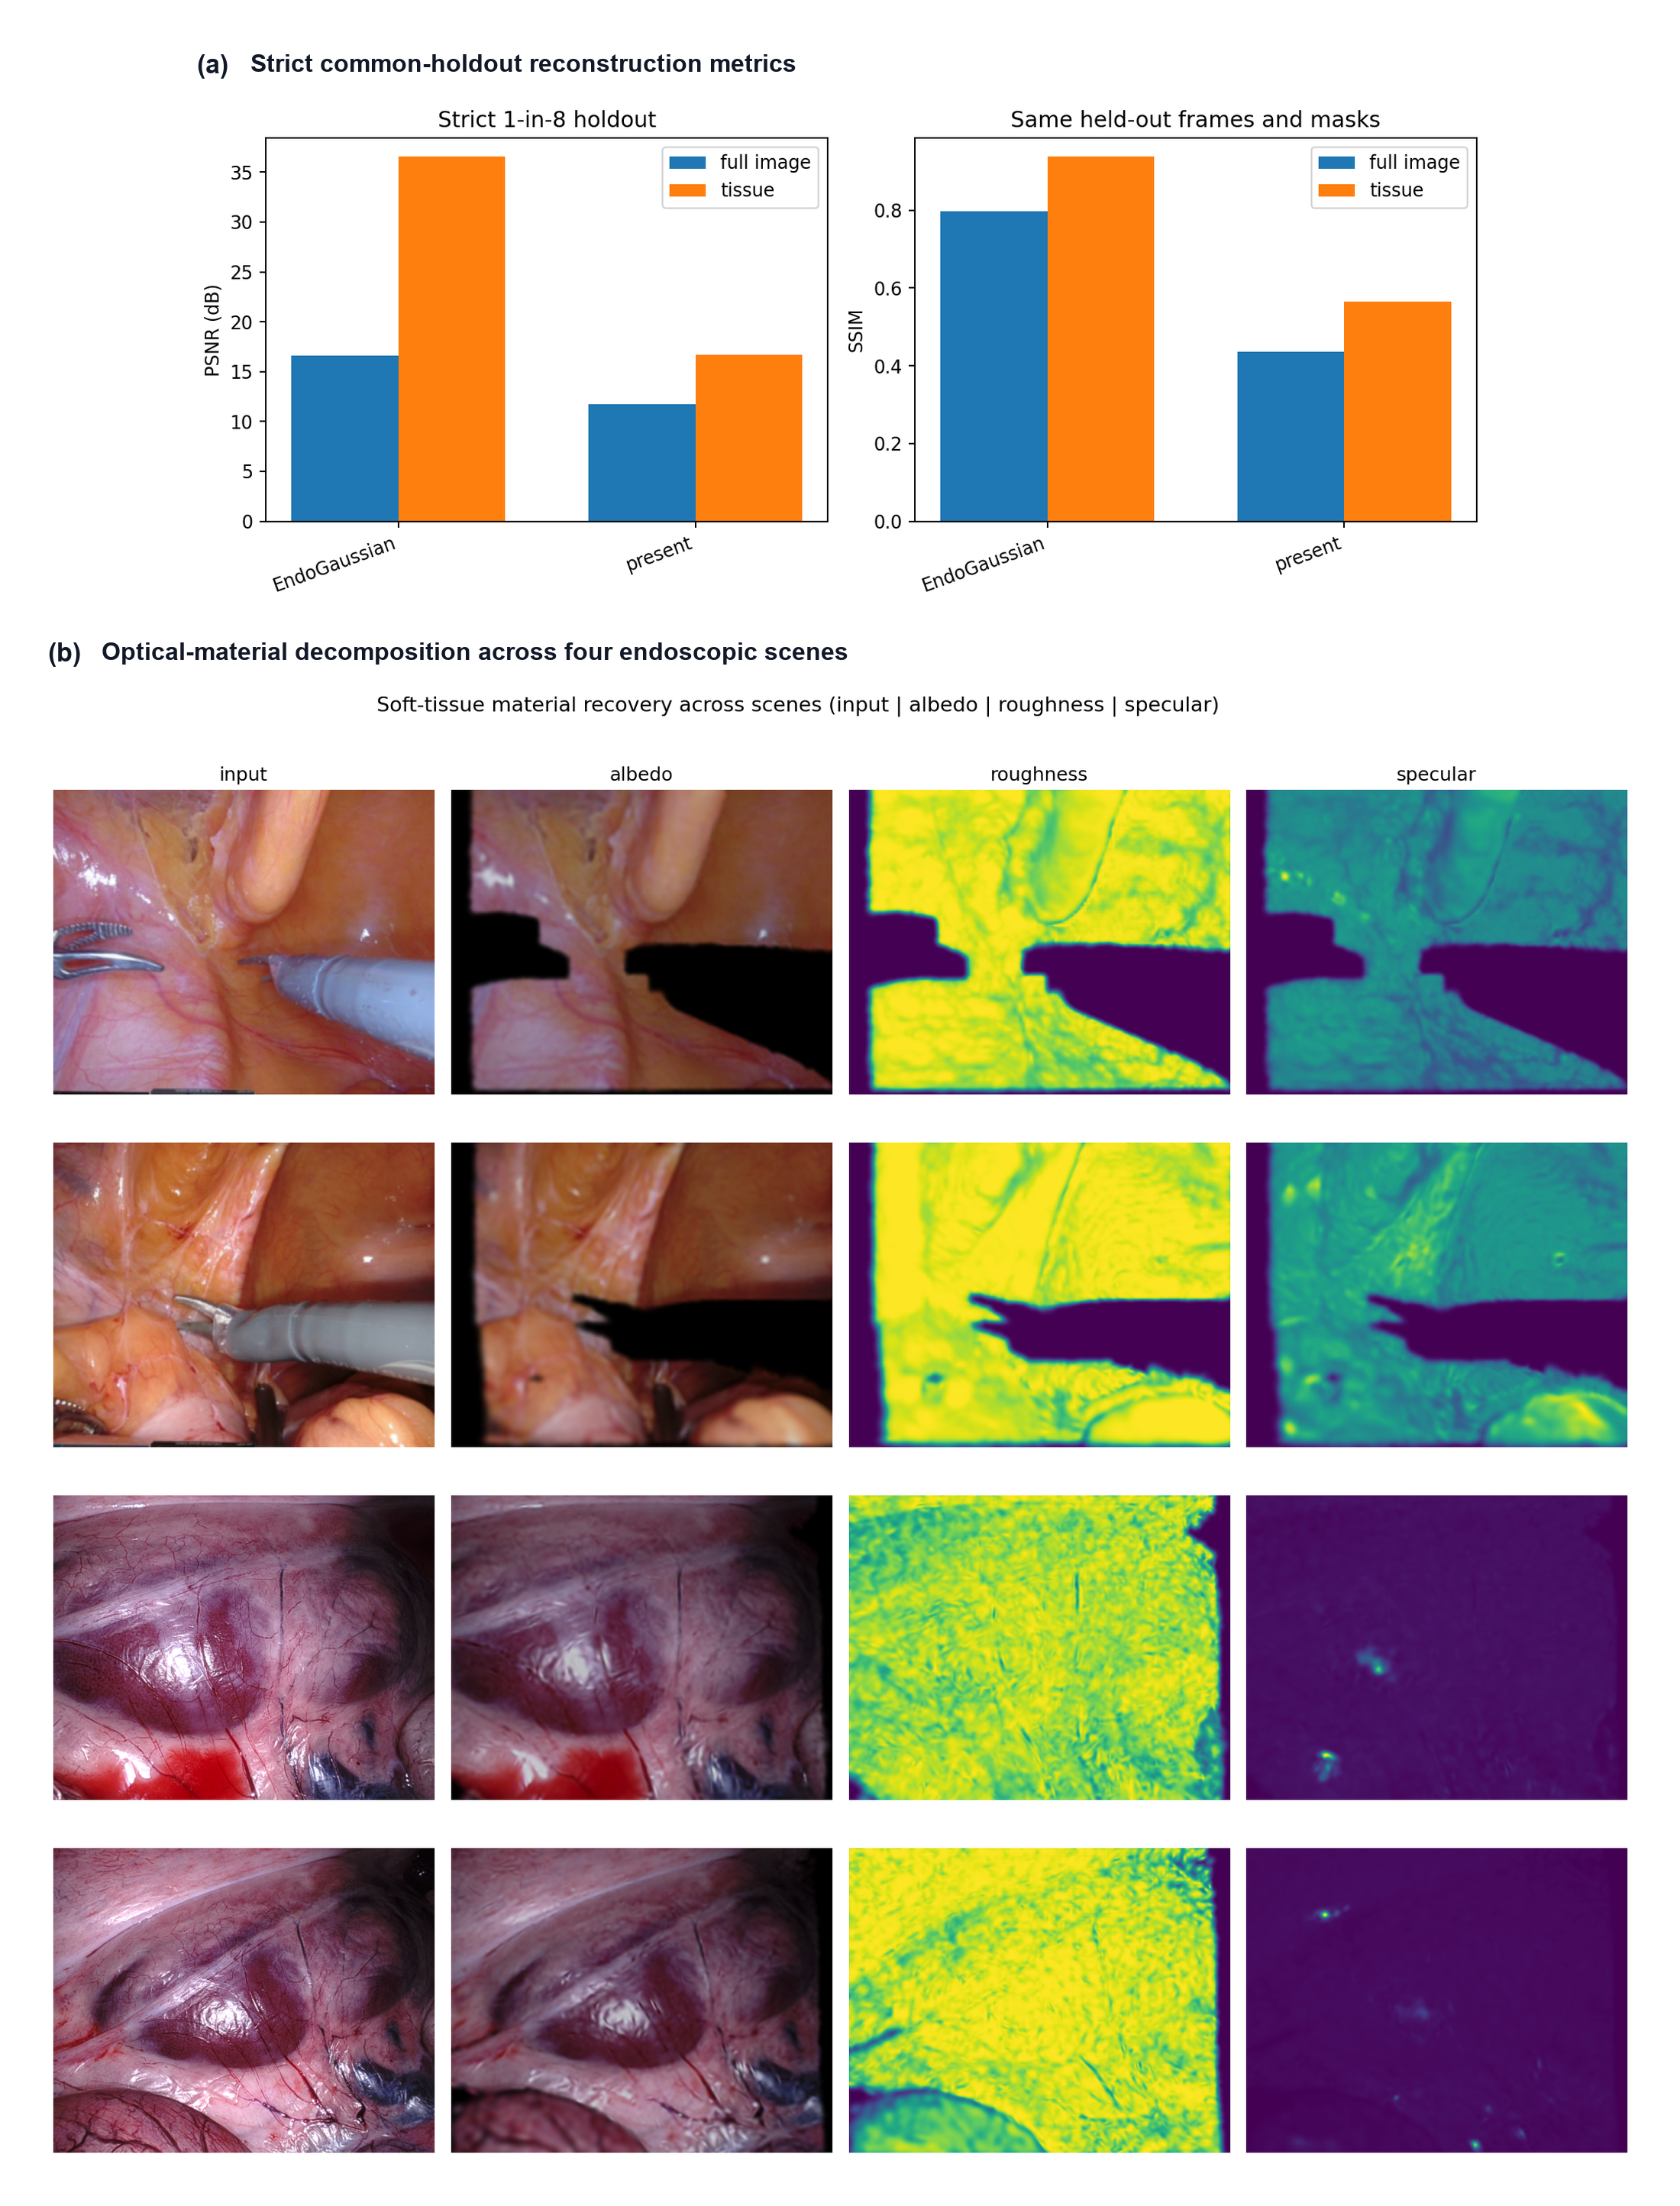
\includegraphics[width=0.94\textwidth]{fig_reconstruction_material_results.png}
\caption{Reconstruction and optical-material evidence. (a) Strict
one-in-eight holdout comparison using identical frames, tissue masks, and
metrics. (b) Input, fitted albedo, roughness, and specular components for
the two EndoNeRF scenes and two SCARED keyframes. EndoGaussian remains
substantially more accurate for novel-view synthesis; the material maps
are estimated outputs of the canonical field.}
\label{fig:reconstruction_material}
\end{figure}


EndoGaussian exceeds the present method by
19.87 dB tissue PSNR and
0.375 tissue SSIM
(Table~\ref{tab:common_holdout}). The gap is consistent across both
scenes. EndoGaussian uses a learned temporal deformation field optimized
for novel-view synthesis, whereas the present representation retains
approximately 6.5--6.8 thousand primitive identities and interpolates
held-out displacement to preserve mechanical correspondence. Optical
decomposition produces spatially varying albedo, roughness, and specular
maps on EndoNeRF and SCARED (Fig.~\ref{fig:reconstruction_material});
these are estimated image-based quantities, not mechanical measurements.

\subsection{Deformation tracking}

\begin{figure}[htbp]
\centering
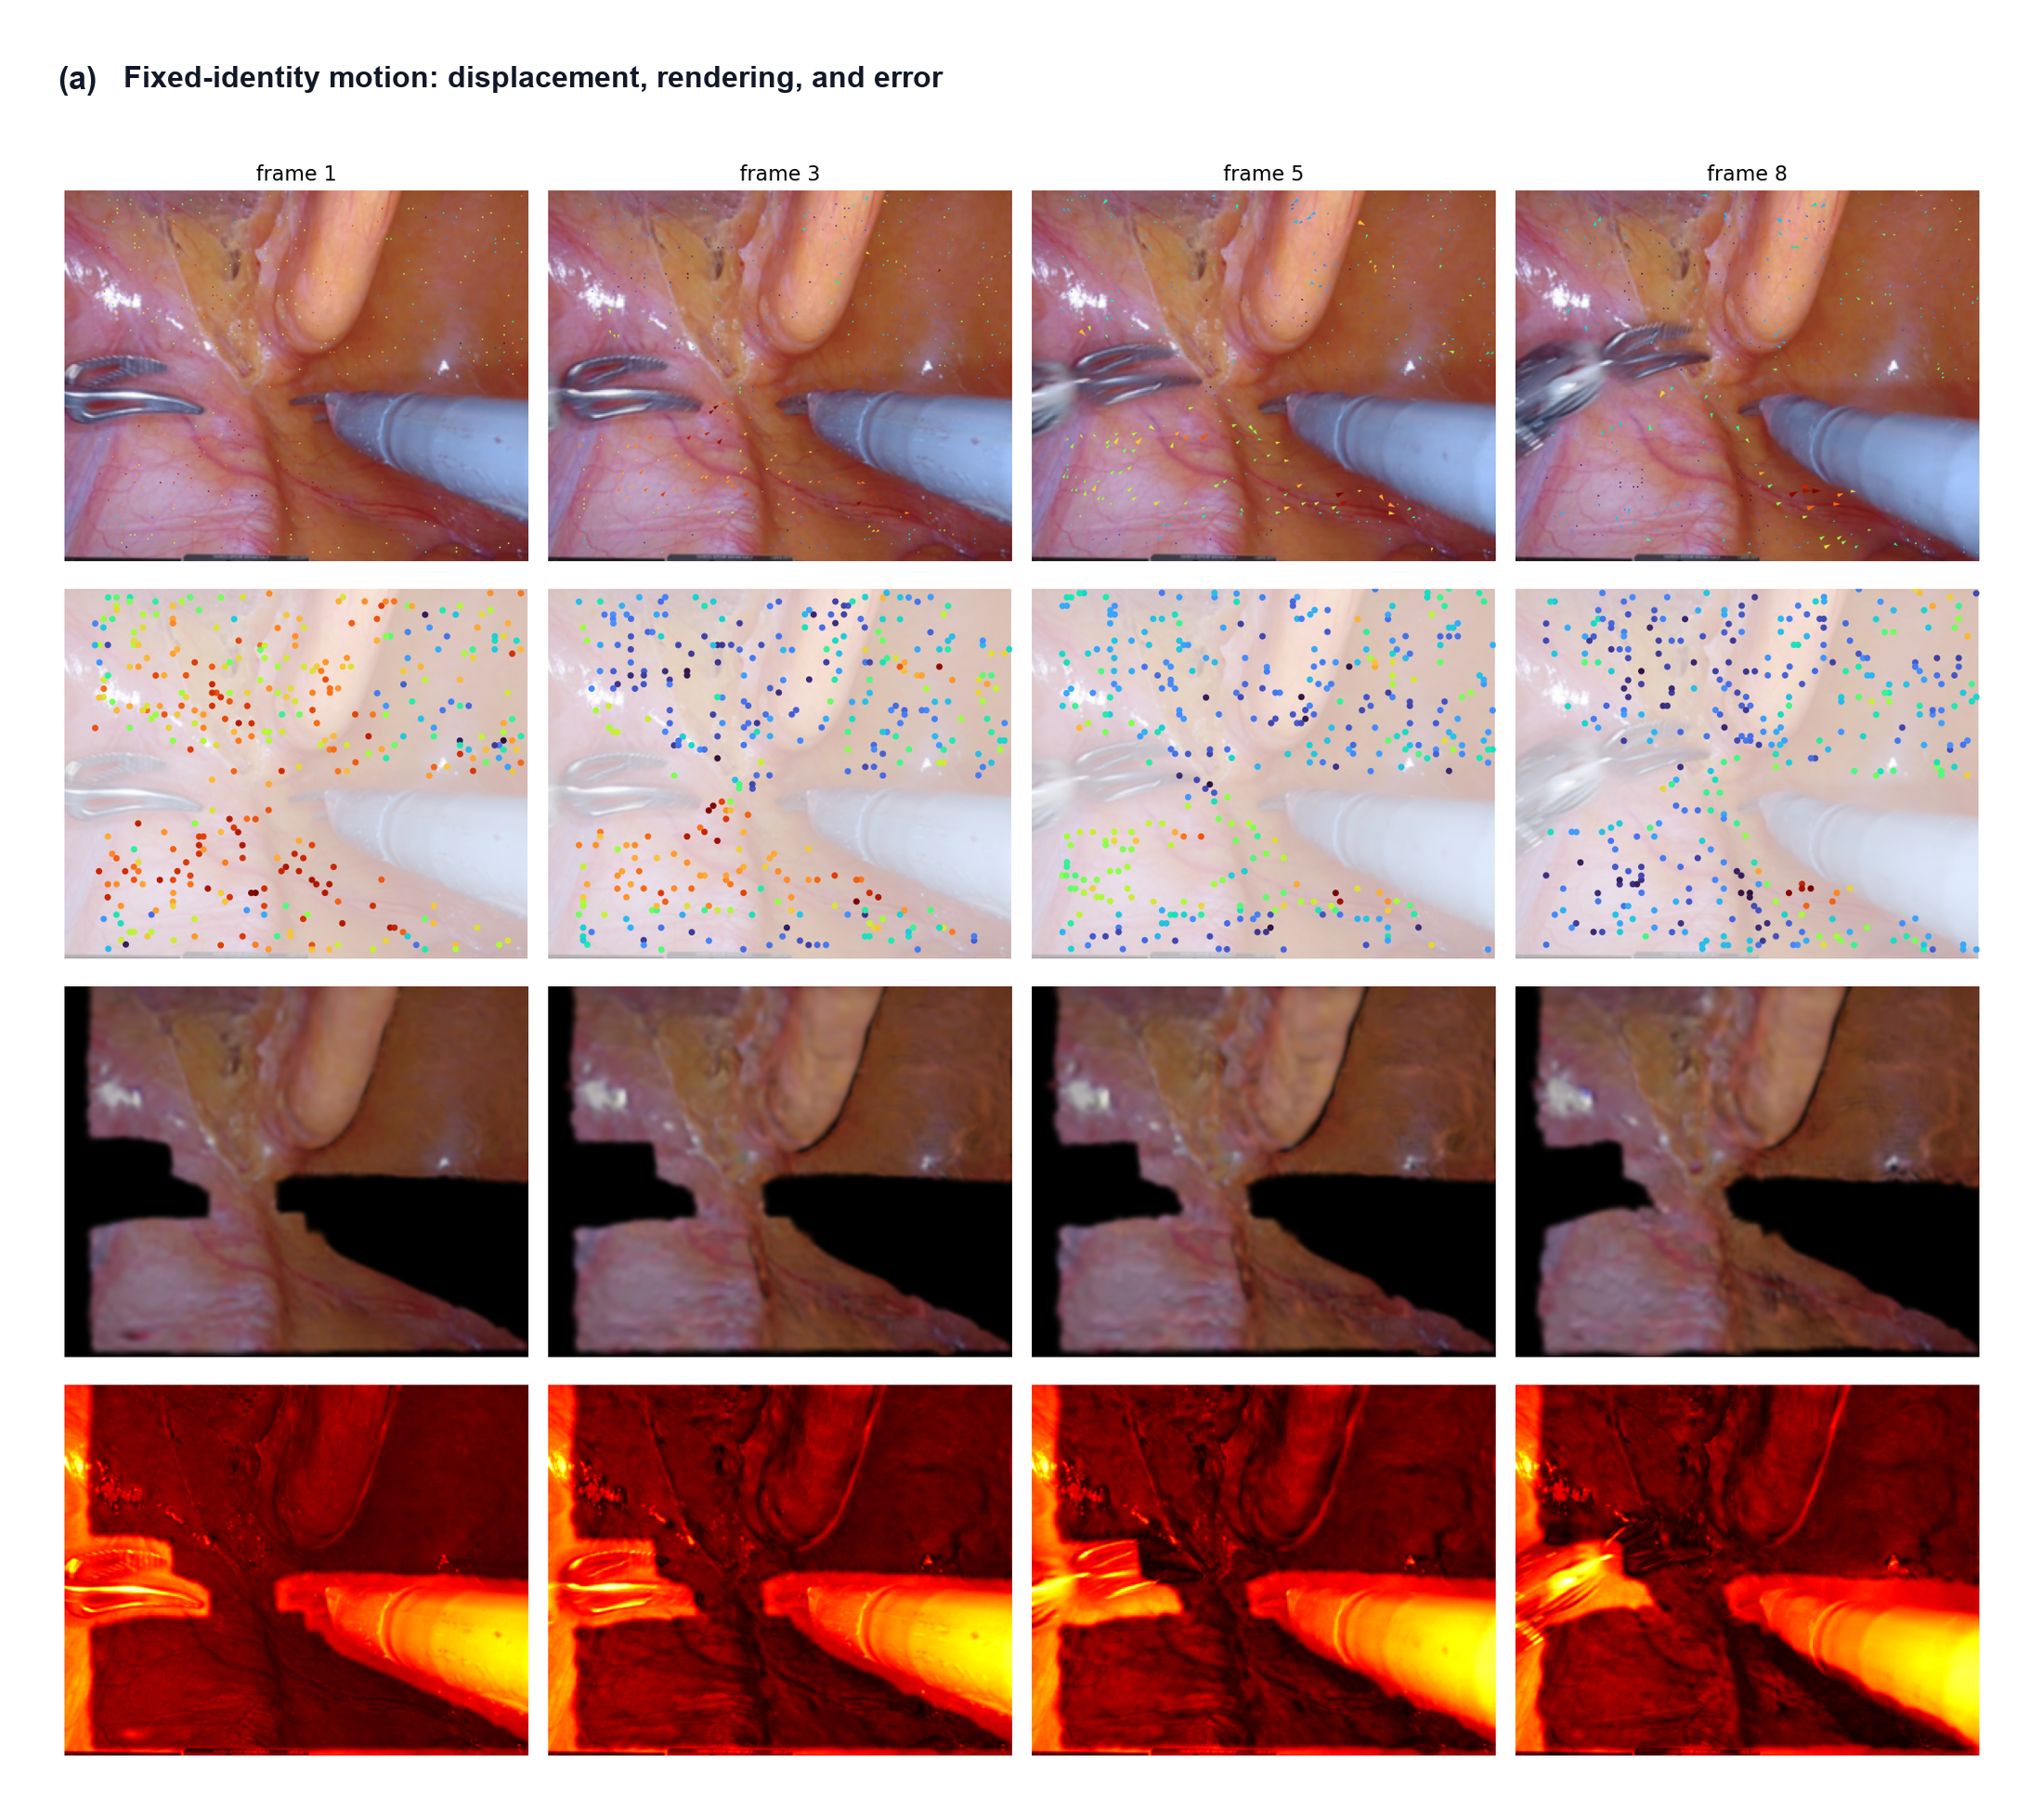
\includegraphics[width=0.94\textwidth]{fig_tracking_results.png}
\caption{Fixed-identity deformation tracking on the EndoNeRF pulling
sequence. Columns show four times; rows show tracked displacement on the
observed frame, displacement magnitude, rendered deformed field, and
photometric error. Primitive identity is retained across time to provide
co-registered surface observations for mechanics.}
\label{fig:tracking_results}
\end{figure}


Fixed-identity tracking follows the contact-centred motion over the tested
sequence (Fig.~\ref{fig:tracking_results}). The inertia-only ablation
diverges at frame 5 with worst-frame loss 37.23. Constant-velocity
initialization, graph regularization, and rollback reduce the corresponding
loss to 1.55 and retain the preceding valid state when re-optimization does
not satisfy the acceptance criterion.

\subsection{Mechanical inversion and physical validation}

\begin{figure}[htbp]
\centering
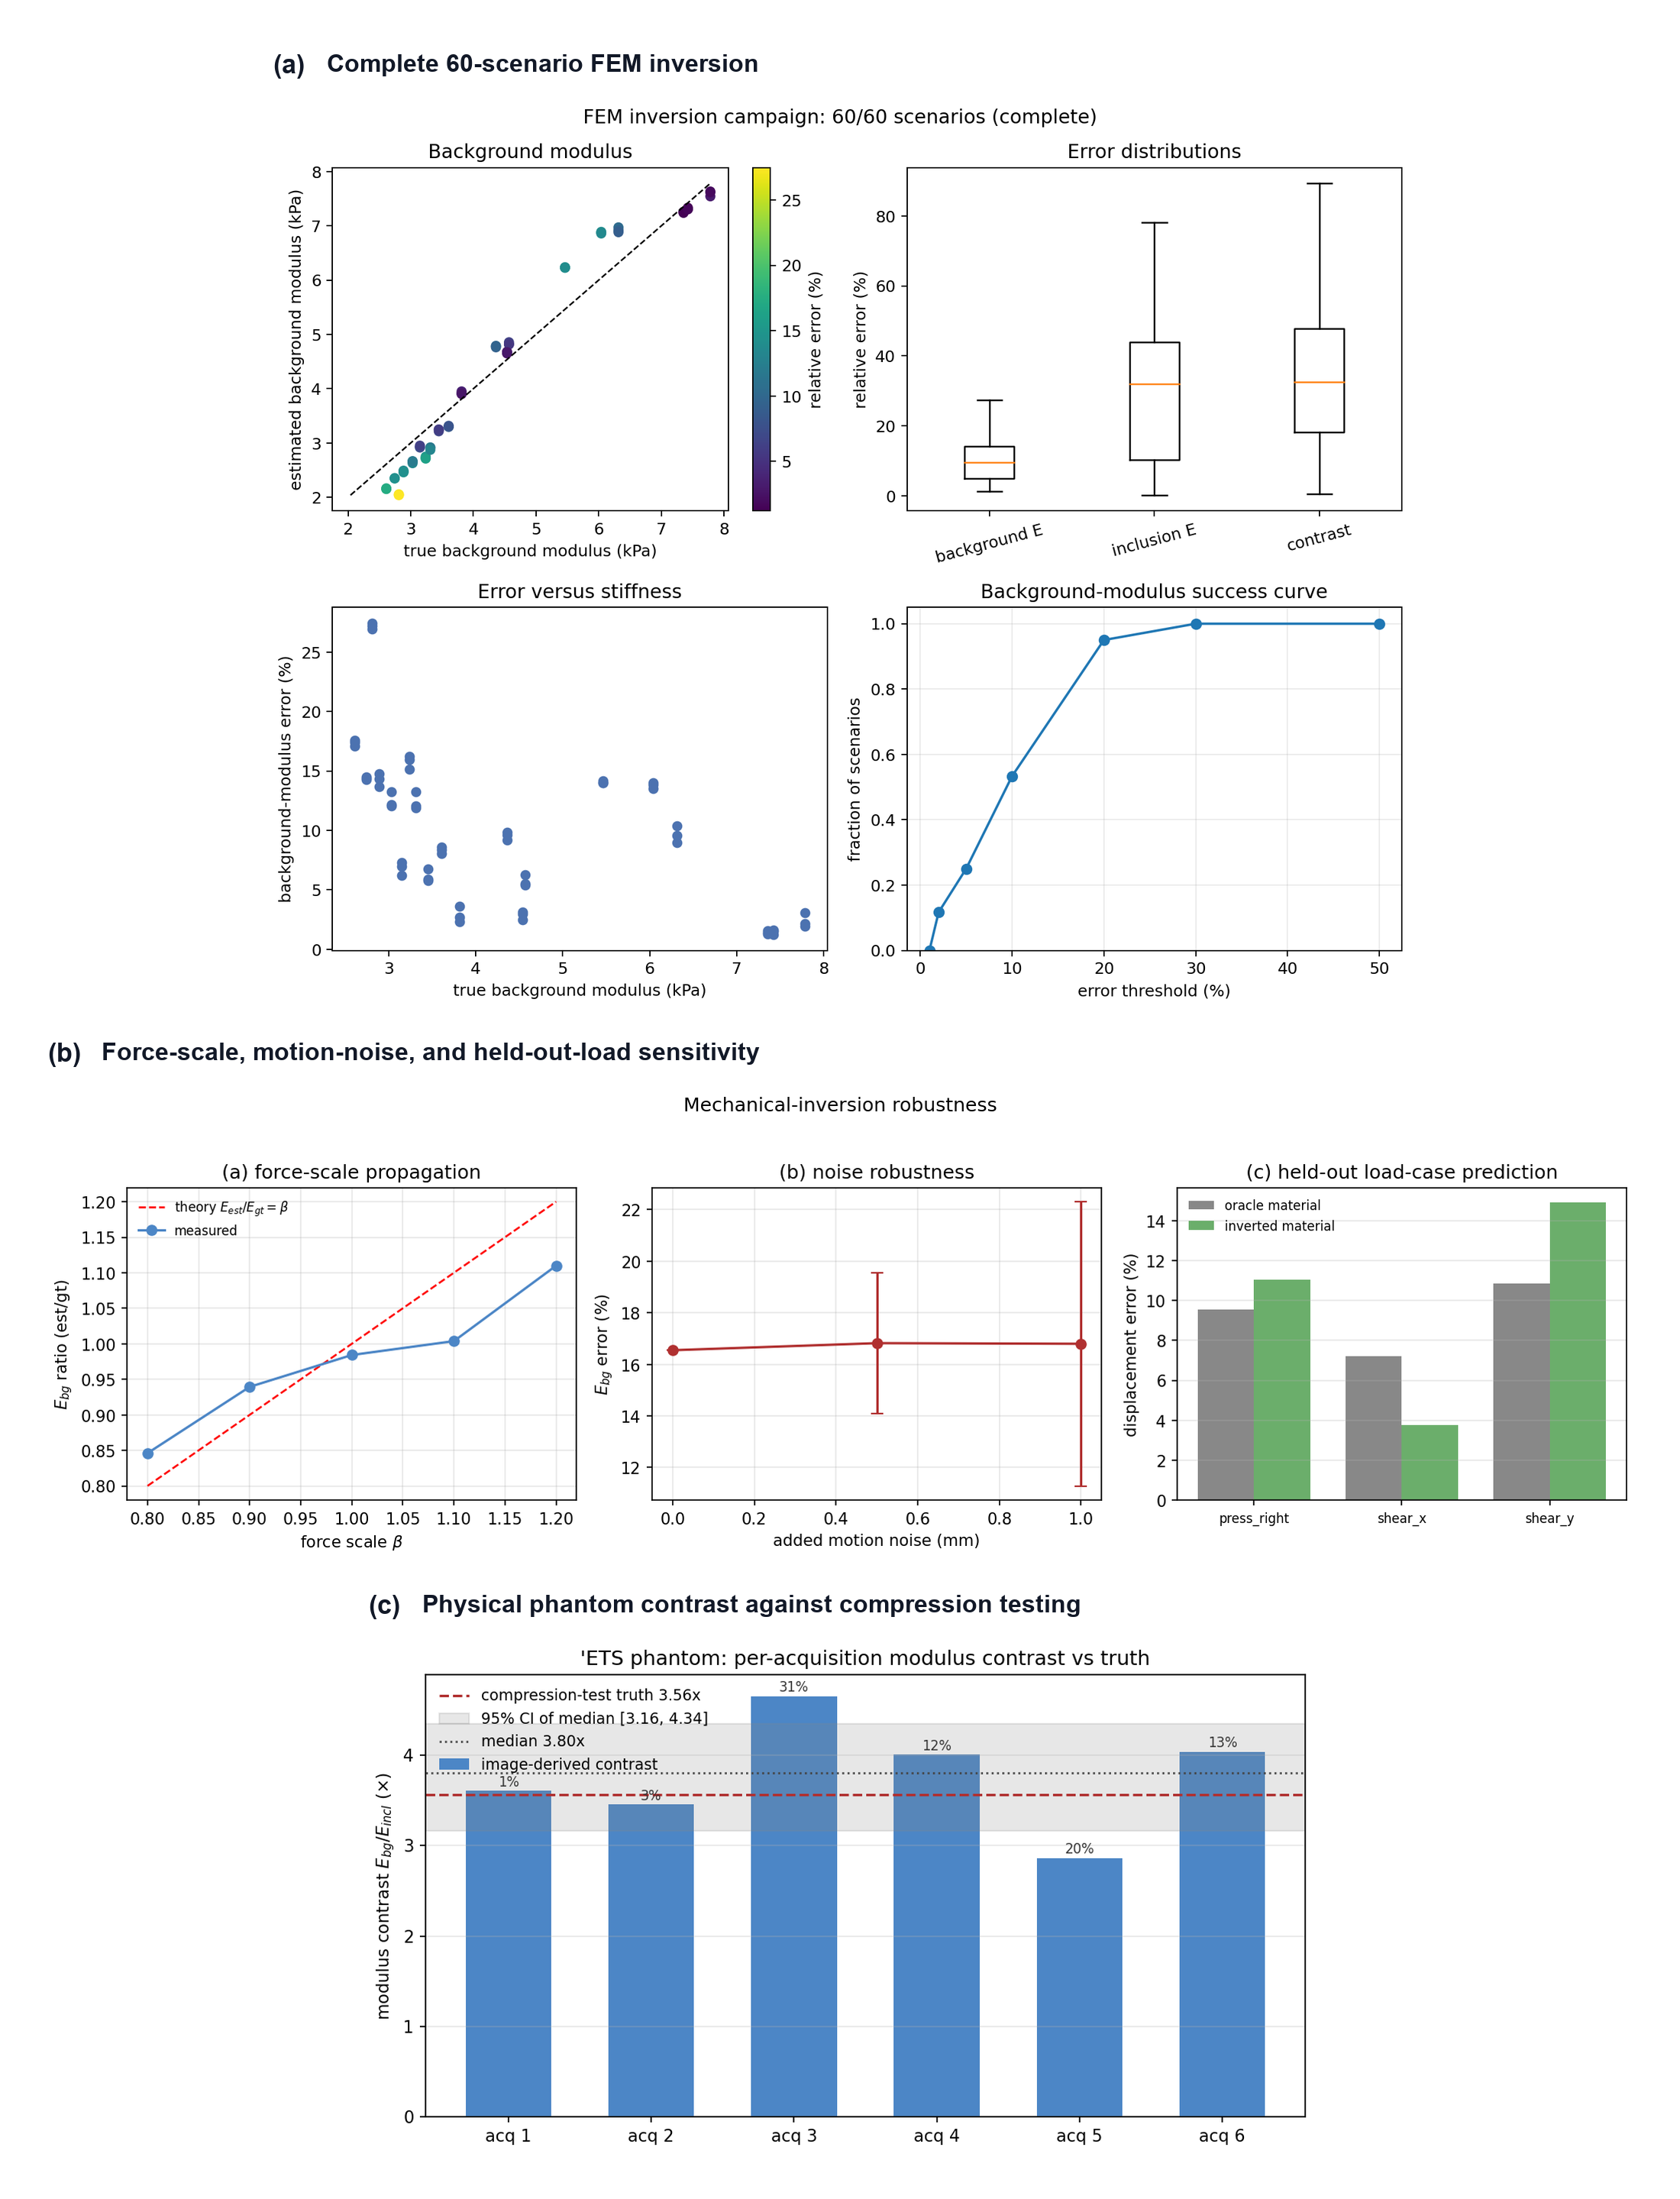
\includegraphics[width=0.94\textwidth]{fig_mechanics_results.png}
\caption{Mechanical validation. (a) Complete 60-scenario FEM inversion,
including modulus agreement, error distributions, stiffness dependence,
and the background-modulus success curve. (b) Force-scale, motion-noise,
and held-out-load sensitivity. (c) Image-derived phantom stiffness
contrast against the independent compression-test reference.}
\label{fig:mechanics_results}
\end{figure}


\begin{table}[htbp]
\centering
\caption{Quantitative mechanical and interface validation.}
\label{tab:mechanical_summary}
\small
\begin{tabular}{p{0.28\textwidth}p{0.24\textwidth}p{0.35\textwidth}}
\toprule
Experiment & Evidence & Result \\
\midrule
Uniform synthetic loop & known force and $E$ & 0.01\% modulus error \\
FEM60 background & measured force, noisy motion &
median 9.6\%; mean 9.9\% \\
FEM60 inclusion & measured force, surface motion &
median 32.0\%; mean 30.1\% \\
FEM60 contrast & common force scale &
median 32.4\%; mean 33.8\% \\
Held-out loads & material fitted on press-left &
11.1\% / 3.7\% / 14.9\% displacement error \\
Force-error propagation & auxiliary error model &
$E_{bg}$ error 4.1$\pm$4.0\%; contrast stable \\
Physical phantom & no absolute force scale &
3.80$\times$ vs 3.56$\times$; 6.9\% error \\
Gaussian--volume map & cross-subject interface &
2,755/7,111 boundary nodes; 38.7\% coverage \\
\bottomrule
\end{tabular}
\end{table}

All 60 predefined FEM scenarios complete under the frozen protocol
(Fig.~\ref{fig:mechanics_results}a). Background modulus is moderately
recovered, but inclusion modulus and contrast remain weak: their median
errors exceed 32\%, and contrast error reaches 89.3\% in the worst case.
The held-out-load experiment uses a representative six-scenario subset;
material fitted on press-left predicts press-right, shear-x, and shear-y
with 11.1\%, 3.7\%, and 14.9\% displacement error, respectively.

The force sweep follows the theoretical scale direction but is not exactly
one-to-one because inversion uses regularization, finite load steps, and
noisy partial-surface observations (Fig.~\ref{fig:mechanics_results}b).
The auxiliary R3D-18 error model is used only in this sensitivity test.
Without force sensing, the physical phantom supports contrast rather than
absolute modulus: the image-derived median is 3.80$\times$ (95\% CI
3.16--4.34) against the compression-test reference of 3.56$\times$
(Fig.~\ref{fig:mechanics_results}c).

\subsection{Gaussian surface to patient-specific volume}
\begin{figure}[htbp]
\centering
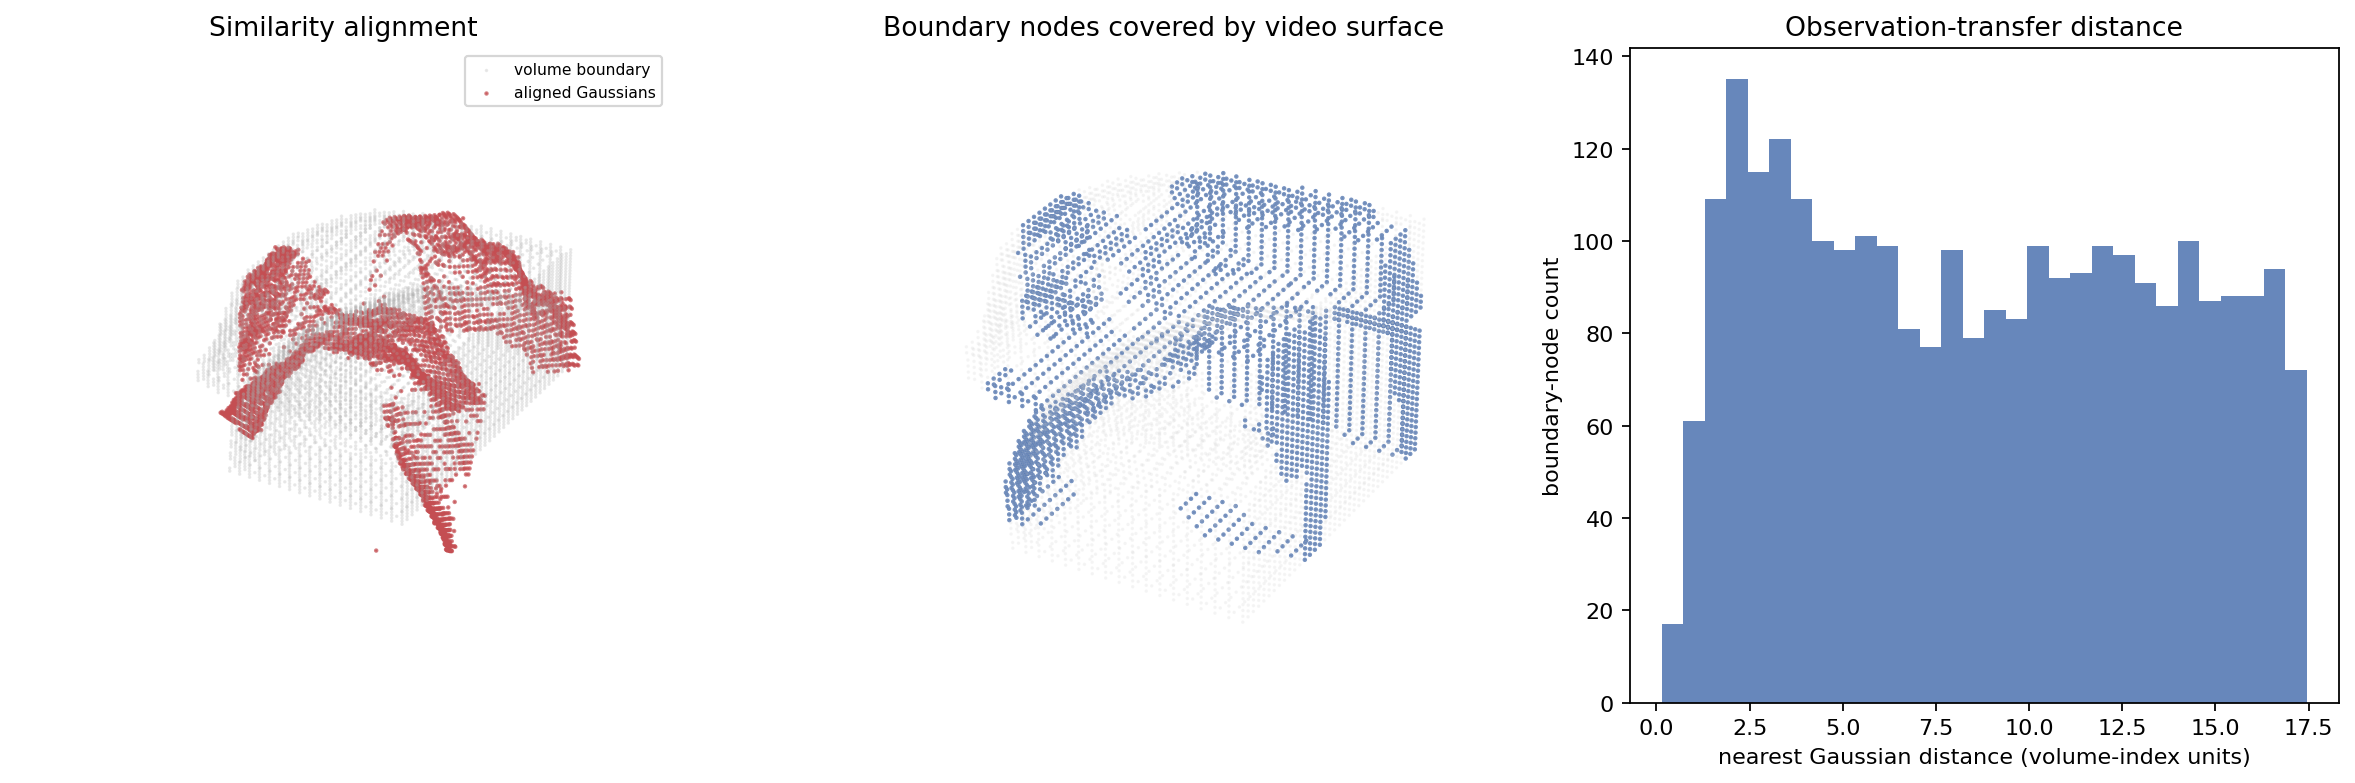
\includegraphics[width=0.92\textwidth]{gaussian_volume_mapping.png}
\caption{Cross-subject computational mapping from the tracked Gaussian
surface to a CT-derived tetrahedral liver volume. Similarity alignment and
inverse-distance interpolation map 2,755 of 7,111 boundary nodes (38.7\%).
The case tests the software interface, not anatomical correspondence or
clinical validity.}
\label{fig:volume_mapping}
\end{figure}

The CT mask yields 28,523 nodes and 149,028 tetrahedra. The normalized
median surface distance after alignment is 0.0237. Because CT spacing is
unavailable and the endoscopic and CT surfaces are from different
subjects, neither physical dimensions nor patient-specific material
parameters are inferred from this experiment.

\subsection{Ablations and uncertainty}
\begin{table}[htbp]
\centering
\caption{Controlled component ablations.}
\label{tab:ablation}
\small
\begin{tabular}{lll}
\toprule
Component & Comparison & Result \\
\midrule
Tissue supervision & tool / depth-valid mask & 11.13 / 36.79 dB \\
Gaussian count & 4,000 / 6,498 / 10,000 & 35.31 / 36.86 / 38.21 dB \\
Temporal model & inertia / proposed tracker & 37.23 / 1.55 loss \\
Parameterization & per-node / two-region & 1.69$\times$ / 3.19$\times$ \\
Forward model & mass--spring / FEM & 82\% forward-model discrepancy \\
\bottomrule
\end{tabular}
\end{table}

The Laplace approximation gives
$\mathrm{std}(\log E_{bg})=1.17$ and
$\mathrm{std}(\log E_{incl})=21.2$, marking the deep inclusion as
weakly identified. Thus, high prediction-interval coverage does not imply
that each modulus is accurately estimated; the interval is dominated by
the poorly constrained inclusion direction.

\section{Discussion}
\label{sec:discussion}
%% ===================================================================

Geometry and reflectance are constrained directly by image and depth
observations. In contrast, Young's modulus is identifiable only when both
deformation and loading are available. The force-provenance analysis
(Sec.~\ref{sec:forcescale}) confirms that uncertainty in the force scale
propagates to absolute modulus but largely cancels in regional stiffness
contrast. Absolute modulus and stiffness contrast should therefore be
interpreted separately.

\paragraph{Example provenance record}
For the pulling sequence, albedo and roughness are marked estimated because
they are fitted to image observations. Tissue class is also marked estimated
because it is selected by an optical heuristic. Young's modulus is marked
assumed (liver prior: median 6\,kPa; 95\% interval 2.3--16.0\,kPa) because
no force was instrumented. Regional stiffness contrast is marked estimated
from deformation, while Poisson's ratio and viscosity retain their
table-derived assumed labels. Simulations based on this sequence should
therefore propagate the prior interval rather than use a single absolute
modulus.

The proposed representation could support simulation of alternative
instrument loads after reconstruction from an intra-operative video.
However, the present evidence establishes technical feasibility rather
than clinical utility. Force-instrumented tissue experiments, prospective
patient data, and task-specific validation are required before the method
can be considered for surgical decision support. Elastography provides the
closest clinical analogue because it also estimates stiffness contrast
from induced deformation \cite{ophir1991}. The phantom experiment indicates
agreement with independent compression testing for this relative
quantity; it does not establish equivalence with clinical elastography.

Any future clinical implementation would also require institutional data
governance, calibrated confidence thresholds, and regulatory evaluation.
The provenance map provides a technical mechanism for exposing the
evidence associated with each parameter, but does not by itself establish
clinical safety.

\paragraph{Reproducibility}\label{sec:repro}
Source code, evaluation scripts, and data-split definitions are available
in the project repository. Every numerical result
reported in this paper is produced by the released end-to-end scripts,
which cover reconstruction, tracking, and inversion on EndoNeRF and SCARED, the FEM
benchmark inversion, the force-provenance analysis, and the phantom audit;
each script writes a machine-readable summary and the corresponding
figures, from which every number in the paper is drawn.

\subsection{Limitations}
\label{sec:threats}
The strict holdout shows that reconstruction accuracy is substantially
below EndoGaussian; fixed surface identity and mechanical coupling do not
compensate for the absence of a learned spatiotemporal deformation field.
Although the FEM analysis covers all 60 predefined scenarios, the
inclusion modulus and contrast remain weakly recovered. The auxiliary
force estimator and its empirical error model are external to the core
twin and have not been independently validated beyond their source
recordings. The \'ETS phantom uses ultrasound rather than
endoscopic colour images, so it validates mechanical contrast but not the optical
reconstruction. The mass--spring surrogate has an 82\% forward error and is
not used to support absolute mechanical estimates on real data. In
addition, the clinical CT experiment contains one de-identified case and
validates geometry construction only. These limitations preclude claims of
clinical performance or absolute-modulus recovery from uninstrumented
endoscopic video.

%% ===================================================================
\section{Conclusion}
\label{sec:conclusion}
%% ===================================================================
The proposed twin couples a canonical Gaussian surface representation with
fixed-correspondence tracking, force-aware mechanical parameterization, and
parameter provenance. Tracked Gaussians provide co-registered surface
motion and regional stiffness contrast for uninstrumented video; absolute
modulus is recovered only in known-force FEM experiments. The force-scale
identity explains why force uncertainty propagates to absolute modulus but
cancels in regional contrast. The common holdout demonstrates that this
mechanically coupled representation does not match the reconstruction
accuracy of EndoGaussian. Across 60 FEM scenarios, median errors are 9.6\%
for background modulus, 32.0\% for inclusion modulus, and 32.4\% for
contrast; the phantom contrast error is 6.9\% against compression testing.
The CT-derived tetrahedral mesh and explicit Gaussian-to-volume map
demonstrate the software interface on one cross-subject case. These
results support the observation-to-simulation framework as a computational
method, but do not establish clinical performance, state-of-the-art
reconstruction, or force-free absolute-modulus recovery. Future work
requires force-instrumented tissue experiments, paired patient-specific
surface and volume data, and prospective evaluation of task-specific
simulation accuracy.



\section*{Abbreviations}
BRDF: bidirectional reflectance distribution function; CI: confidence
interval; CT: computed tomography; FEM: finite-element method; MPM:
material point method; NVS: novel-view synthesis; PSNR: peak
signal-to-noise ratio; RGB: red, green, and blue; SCARED: Stereo
Correspondence and Reconstruction of Endoscopic Data.

\section*{Declarations}

\subsection*{Ethics approval and consent to participate}
The public EndoNeRF, SCARED, finite-element benchmark, and \'ETS phantom
datasets do not involve identifiable human subjects. The hospital computed
tomography images are de-identified retrospective scans provided by Henan
Provincial People's Hospital for geometry-source validation; no
identifiable patient information is reported. The name of the responsible
ethics committee and the approval or waiver reference must be inserted
after confirmation by the data-providing institution.

\subsection*{Consent for publication}
Not applicable. The manuscript does not contain data from any identified individual person.

\subsection*{Availability of data and materials}
Source code, frozen data splits, evaluation scripts, and machine-readable
result summaries are available at
\url{https://github.com/liranyang123456-commits/soft-tissue-digital-twin}.
EndoNeRF, SCARED, the FEM benchmark, and the \'ETS phantom are public
datasets cited in this article. The de-identified hospital CT images are
not publicly redistributed under the data-providing institution's
governance.

\subsection*{Competing interests}
The authors declare that they have no competing interests.

\subsection*{Funding}
This work was supported by the National Natural Science Foundation of China (6240074117), the Henan University of Technology Young Backbone Teachers Training Program (21421329), the Open Project Program of the State Key Laboratory of Virtual Reality Technology and Systems (VRLAB2023C03), and the Cultivation Project of Tuoxin Team in Henan University of Technology (2024TXTD18). The funders had no role in study design, data collection, analysis, decision to publish, or preparation of the manuscript.

\subsection*{Authors' contributions}
RL conceived the study, developed the method, wrote the software, and drafted the manuscript. HM contributed the algorithm, software, and validation. ZL contributed validation, formal analysis, and multi-view evaluation. NW contributed clinical data curation and anatomical review. All authors read and approved the final manuscript.

\subsection*{Acknowledgements}
The authors thank Henan Provincial People's Hospital for providing the de-identified clinical computed tomography data used for the geometry-source validation.

\bibliographystyle{spmpsci}
\bibliography{references}


\end{document}
